
\newcommand{\prexo}{\emph{pre\_exodus \,}}
\newcommand{\bc}{\emph{bc-file \,}}
\newcommand{\head}{\emph{header-file \,}}

%%
%%############################
\chapter{Fluid Tutorial with \prexo and Cubit}
\label{tut_fluid_preexo:chap}
%Flow around a Cylinder - Von Karman vortex street

%%
%%============================
\section{Introduction}
In this tutorial we want to simulate the incompressible flow past a circular cylinder.
For further details and references we refer the reader to:\\
W.A. Wall, PhD thesis, 1999
(available under \texttt{/lnm/literature/1999/})
\begin{figure}[h]
\begin{center}
 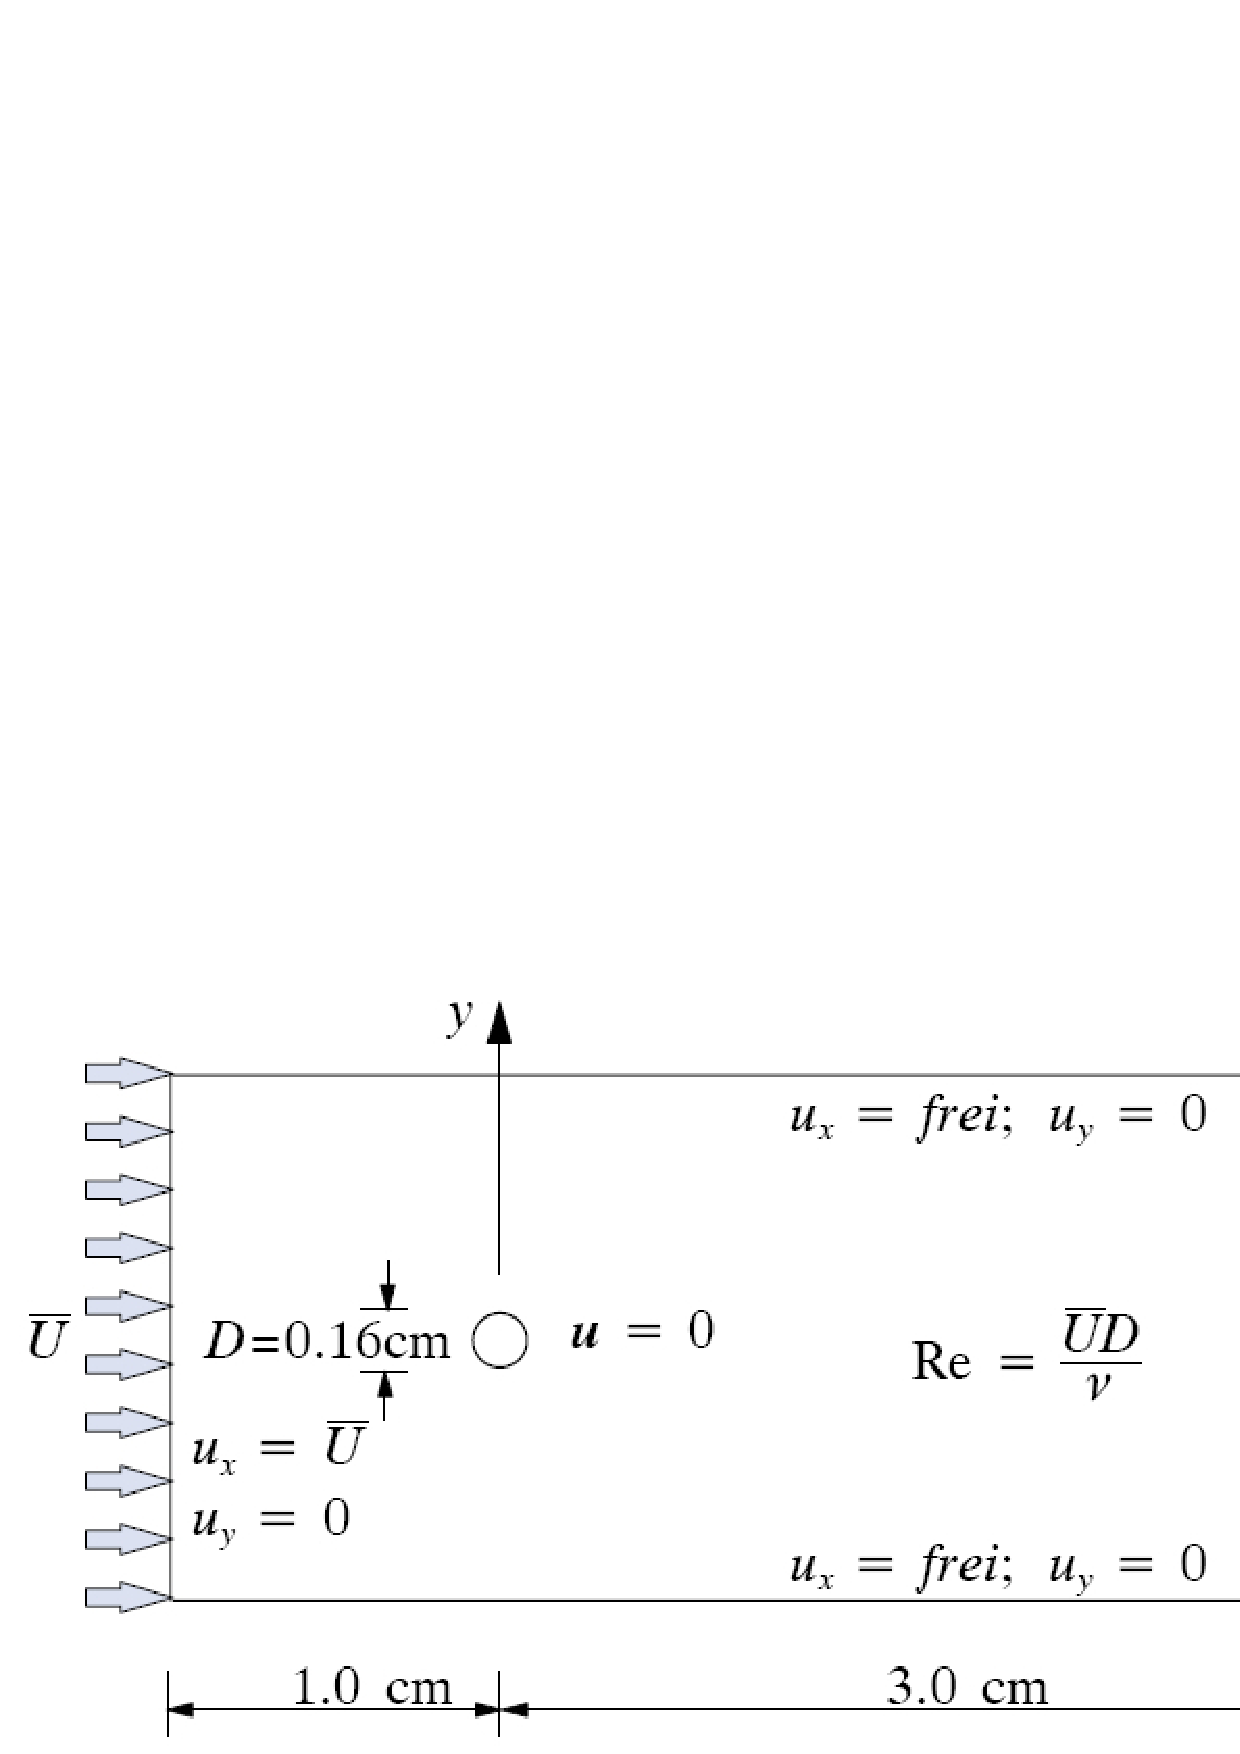
\includegraphics[scale=0.35]{pics/tut_fluid_problem}
 \caption{Problem definition and geometrical setup (with friendly permission ;-))}
\label{fig:tut_fluid_preexo_setup}
\end{center}
\end{figure}

%%
%%============================
\section{\baci{} Setup}

In order to use \baci{} for your special purposes (here: Fluid Flow), you have
to do a kind of setup first. 

\begin{itemize}
\item Execute the following command in the console (in the \baci{} directory):\\
\emph{./do-configure}\\
This creates the \texttt{Makefile} needed for compiling the code
in the following steps. 
\item Now simply run \emph{make -j 2}.
\item It will take about twenty minutes to compile Baci
\end{itemize}
This created everything necessary for BACI to solve your specific
problem.


%%
%%============================
\section{Preprocessing}

\subsection{Creating the Geometry with Cubit}
We will use Cubit version 12.0 for creating the geometry and the mesh. Cubit 12.0 can be executed by \newline
\texttt{/lnm/programs/cubit12/cubit}. Within Cubit, open the Journal-Editor (\emph{Tools}$\to$\emph{Journal
Editor}), paste the text below and press \emph{play}. If the geometry couldn't be created, try to set the editor to 
'Translate to Cubit commands' first and retry. After successful geometry and mesh creation, export everything to an Exodus-file of your choice via \emph{File}$\to$\emph{Export...}.

\begin{small} \begin{verbatim}
$***********************
$  preliminaries     
$***********************

reset
set geometry engine acis

$***********************
$  create geometry     
$***********************

$ define geometric parameters

$ in cm

# {fluid_length = 4.0} $ x-direction
# {fluid_width = 2.0} $ y-direction
# {cyl_radius = 0.08}
# {cyl_offset = 1.0}


$ create domain 
create vertex {-cyl_offset} {fluid_width/2.0} 0
create vertex {-cyl_offset} {-fluid_width/2.0} 0
create vertex {fluid_length-cyl_offset} {fluid_width/2.0} 0
create vertex {fluid_length-cyl_offset} {-fluid_width/2.0} 0
create vertex 0 0 0
create vertex {cyl_offset} {fluid_width/2.0} 0
create vertex {cyl_offset} {-fluid_width/2.0} 0

create curve vertex 1 vertex 5
create curve vertex 5 vertex 6
create curve vertex 6 vertex 1

create curve vertex 10 vertex 2
create curve vertex 2 vertex 8

create curve vertex 12 vertex 7
create curve vertex 7 vertex 13

create curve vertex 15 vertex 9

create curve vertex 18 vertex 3
create curve vertex 3 vertex 4
create curve vertex 4 vertex 17

create surface curve 3 1 2
create surface curve 1 4 5
create surface curve 5 6 7
create surface curve 7 8 2
create surface curve 8 9 10 11


create vertex 0 0 0
create vertex 0 {cyl_radius} 0
create vertex {cyl_radius} 0 0

create curve arc center vertex 24 25 26 {cyl_radius} full
create surface curve 17
delete vertex 24 25 26

subtract volume 6 from volume 1 2 3 4

imprint volume all
merge volume all

$***********************
$ create mesh         
$***********************

# {numele_past_x = 37}
# {numele_past_y = 34}
# {numele_cyl_x = 30}
# {numele_inflow = 22}
# {numele_radial = 50}


group "radial" add curve 19 20 23 26

curve 9 scheme equal interval {numele_past_x}
curve 10 scheme equal interval {numele_past_y}
curve in group radial scheme equal interval {numele_radial}
curve 3 6 scheme equal interval {numele_cyl_x}
curve 4 scheme equal interval {numele_inflow}

$ apply bias for better mesh
curve 19 scheme bias factor 0.9 start vertex 1 interval {numele_radial}
propagate curve bias volume all

curve 20 scheme bias factor 0.9 start vertex 6 interval {numele_radial}
propagate curve bias volume all

curve 23 scheme bias factor 0.9 start vertex 2 interval {numele_radial}
propagate curve bias volume all

curve 26 scheme bias factor 0.9 start vertex 7 interval {numele_radial}
propagate curve bias volume all


mesh surface all


$***********************
$ boundary conditions 
$***********************

reset block
block 1 surface all

nodeset 1 curve 4
nodeset 1 name "inflow"

nodeset 2 curve 3 9
nodeset 2 name "top"

nodeset 3 curve 6 11
nodeset 3 name "bottom"

nodeset 4 curve 18 21 24 27
nodeset 4 name "cylinder"

nodeset 5 vertex 1 2
nodeset 5 name "corners"
\end{verbatim} \end{small}

When Cubit version 11.0 (\texttt{/lnm/programs/cubit.11.0/cubit}) is used for 
creating geometry and mesh, you have to adapt some of the previous commands,
since numbering of entities changed between Cubit versions!

The generated mesh should look like this:
\begin{figure}[H]
 \begin{center}
  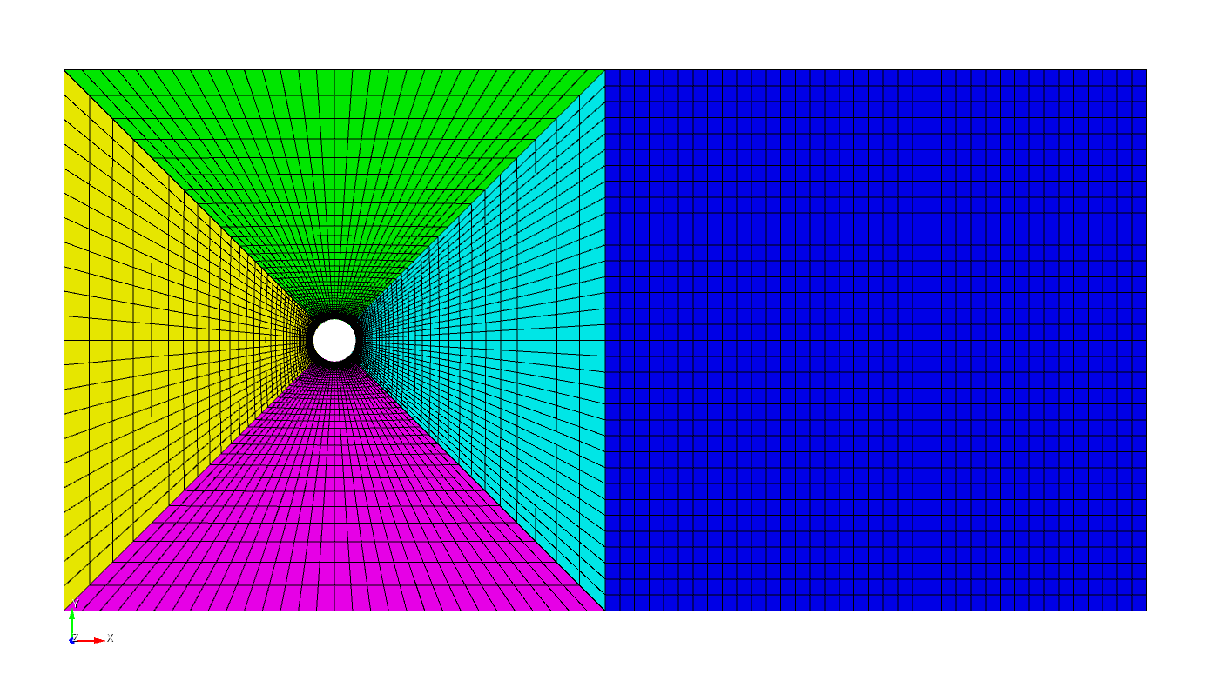
\includegraphics[width=0.95\textwidth]{pics/tut_fluid_mesh}   
  \caption{Mesh for a flow past a circular cylinder.}
  \label{fig:domainDecomposition}
\end{center}
\end{figure}

\section{Working with \prexo and \baci{}}

\prexo is a C++ code embedded into the \baci{} environment. It is meant to
transfer a given mesh into a \baci{}-readable input file.

\subsection{Preliminaries}

If not already done, compile \prexo via \begin{verbatim}make pre_exodus\end{verbatim} after 
configuring \baci{} in the usual way.

\subsection{General Procedure of Creating a Valid \baci{} Input File}
With a given mesh including some nodal clouds to apply conditions to you need
another text-file {(\bc)} where you specify, what you would like to do with
it. It contains for example the specific element declaration (fluid, structure,
parameters, etc.) and the particular boundary condition such as Dirichlet or
Neumann. Finally, a \head consists of general parameters such as
solvers, algorithmic parameters, etc. Those three files are merged by \prexo
into an input file for \baci{}. This file is then \emph{automatically} validated
using all available \baci{} validation and is therefore likely to run.

Sure, you usually do not have already a proper \head and matching \bc. By
typing
\begin{center}
  \verb|./pre_exodus --exo=yourmesh.e|
\end{center}
you get two preliminary files
'default.head' and 'default.bc'. The first contains the currently valid header
parameters with default values and commented options which you can edit to
adapt it to your means. Similarly, 'default.bc' consists of all your mesh
entities and a list of all currently valid conditions. See next section for
details how to work with them and how to create valid input files.


\subsection{Adapting the \head}
Open the previously created \head 'default.head' and edit the following entries as shown below.
\begin{itemize}
 \item \verb|PROBLEM TYP|

 \verb|PROBLEMTYP Fluid|
 \item \verb|FLUID DYNAMIC|

 \verb|NUMSTEP 20|

 \verb|TIMESTEP 0.01|

 \item \verb|MATERIALS|

 insert the following line after \verb|------MATERIALS| in order to define your material parameters: \newline
 \verb|MAT 1 MAT_fluid DYNVISCOSITY 0.004 DENSITY 1.0|

 \item \verb|CURVE 1|

 insert the following line after \verb|------CURVE 1| in order to define a time curve: \\
 \verb|CURVE1 on EXPR FUNC 0.5*(sin((t*pi/0.1)-(pi/2)))+0.5  t1 0.0 t2 0.1|
 
\end{itemize}
Save the file under a different name of your choice.

\subsection{Adapting the \bc}
Open the previously created \bc 'default.bc' and edit your boundary conditions as shown below.


 \begin{small} \begin{verbatim}
Element Block, named: 
of Shape: SHELL4
has 7058 Elements
*eb1="ELEMENT"
sectionname="FLUID"
description="MAT 1 NA Euler"
elementname="FLUID2"

Node Set, named: inflow
Property Name: none
has 23 Nodes
*ns1="CONDITION"
sectionname="DESIGN LINE DIRICH CONDITIONS"
description="1 1 0 0 0 0  1.0 0.0 0.0 0.0 0.0 0.0  1 none none none none none  0 0 0 0 0 0"

Node Set, named: top
Property Name: none
has 68 Nodes
*ns2="CONDITION"
sectionname="DESIGN LINE DIRICH CONDITIONS"
description="0 1 0 0 0 0  0.0 0.0 0.0 0.0 0.0 0.0  none none none none none none  0 0 0 0 0 0"

Node Set, named: bottom
Property Name: none
has 68 Nodes
*ns3="CONDITION"
sectionname="DESIGN LINE DIRICH CONDITIONS"
description="0 1 0 0 0 0  0.0 0.0 0.0 0.0 0.0 0.0  none none none none none none  0 0 0 0 0 0"

Node Set, named: cylinder
Property Name: none
has 116 Nodes
*ns4="CONDITION"
sectionname="DESIGN LINE DIRICH CONDITIONS"
description="1 1 0 0 0 0  0.0 0.0 0.0 0.0 0.0 0.0  none none none none none none  0 0 0 0 0 0"

Node Set, named: edges
Property Name: none
has 2 Nodes
*ns5="CONDITION"
sectionname="DESIGN POINT DIRICH CONDITIONS"
description="1 1 0 0 0 0  1.0 0.0 0.0 0.0 0.0 0.0  none none none none none none  0 0 0 0 0 0"
 \end{verbatim} \end{small}
Save the file under a different name of your choice.

\subsection{Creating a \baci{} input file with \prexo}
The previously created files have to be merged to a \baci{} input file in oder 
to solve the problem. We will use \prexo for this purpose. Open a terminal 
and execute the following command:
\begin{center}
  \verb|./pre_exodus --exo=/meshpath/yourmesh.exo --head=/headpath/headerfile.head|
  \verb|	--bc=/bcpath/bcfile.bc --dat=/datpath/datfile.dat|
\end{center}
Where the filenames and their paths have to be replaced according to how you have named and where you have saved them.
\prexo will output a dat-file to the path you specified above.


\subsection{Running a Simulation with \baci{}}
\label{tut_fluid_preexo:baci}
To start the solver use the call 
\begin{center}
	\verb|./baci-release [inputdirectory]/datfile.dat [outputdirectory]/outputprefix|
\end{center}
(in the \baci{}-directory). You may have to adapt the name of the executable 
in this command. The prefix that you have chosen before will 
be applied to all output files that \baci{} generates.


\section{Postprocessing}

You can postprocess your results with any vizualization software you like. In this tutorial, we choose \emph{Paraview}. 

\subsection{Filtering result data}
\begin{itemize}
\item Before you can admire your results, you have to generate a filter 
which converts the generic binary \baci{} output to the desired format.
Starting from the \baci{} directory, execute \texttt{make post\_drt\_ensight}.
\item The filter should now be available in your \baci{} directory. Filter your results with
the call (inside the \baci{} directory): \texttt{./post\_drt\_ensight -\,-file=[outputdirectory]/outputprefix} 
\item Further options of the filter program are made visible by the command \texttt{post\_drt\_ensight --help}
\end{itemize}

\subsection{Visualize your results in Paraview}
\begin{itemize}
\item After the filtering process is finished open \emph{paraview} by typing \newline
\texttt{/lnm/programs/paraview-3.6.1-Linux-i686/bin/paraview \&}
\item \emph{File$\to$Open} and select the filtered \emph{*.case}
file: \emph{outputprefix.case}
\item choose \emph{LittleEndian} instead of \emph{LittleEndian} and press \emph{Apply} to activate the display.
\item choose time step $19$ ($=0.2$) in the top menu bar 
\item At \emph{Color by} you can choose now between \emph{pressure} and \emph{velocity (Magnitude, X, ...)}. Choose \emph{velocity (X)}!
\item in the \emph{Display} tab (section \emph{Color}) press \emph{Rescale to Data Range}. 
\item For the scale, press \emph{Edit Color Map}, choose the tab \emph{Color legend} and activate \emph{Show color legend}.
You receive a visualization of the x-velocity field, which should look like Fig. \ref{fig:FlowPastCylinder_x-velocity}.
\end{itemize}

\begin{figure}[H]
 \begin{center}
  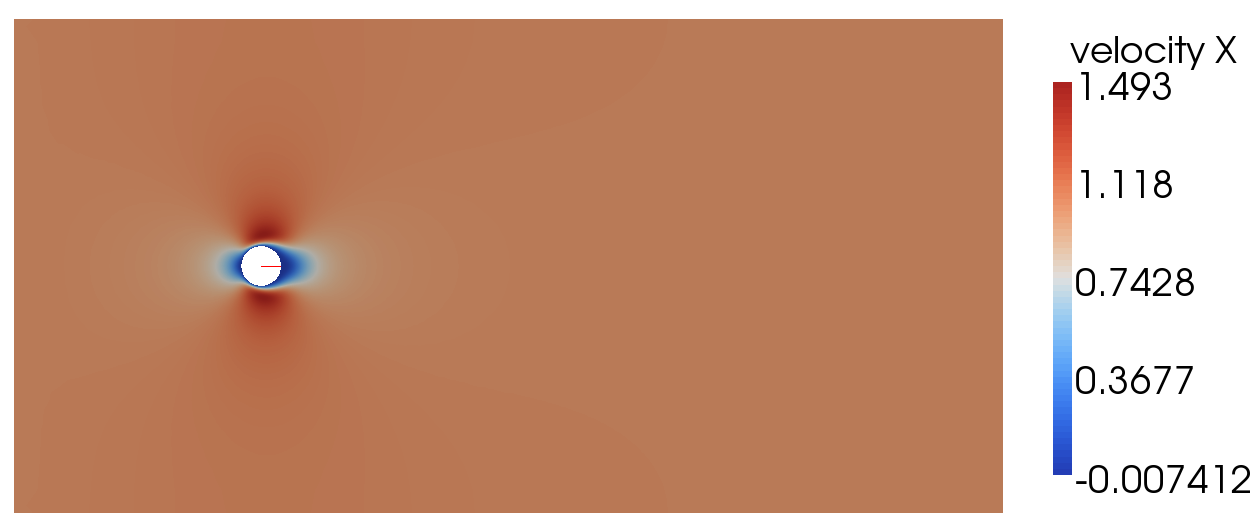
\includegraphics[width=0.95\textwidth]{pics/tut_fluid_xvel.png}   
  \caption{x-velocity for a flow past a circular cylinder.}
  \label{fig:FlowPastCylinder_x-velocity}
\end{center}
\end{figure}
